\documentclass[handout]{beamer}

\usetheme[progressbar=frametitle]{metropolis}
\metroset{block=fill}

\subtitle{NTIN071 Automata and Grammars}
\author{Jakub Bulín (KTIML MFF UK)}

\date{Spring 2025\\ 
    \vspace{1in} 
    \begin{flushleft}
        \it \footnotesize * Adapted from the Czech-lecture slides by Marta Vomlelová with gratitude. The translation, some modifications, and all errors are mine.
    \end{flushleft}
}

%% packages

\usepackage{amsmath}
\usepackage{amssymb}
\usepackage{amsthm}
\usepackage{cancel}
\usepackage{color}
\usepackage{colortbl}
\usepackage{forest}
\usepackage[utf8x]{inputenc}
\usepackage{multicol}
\usepackage{multirow}

%% colors
\definecolor{Gray}{gray}{0.9}

%% TikZ
\usepackage{tikz}
    \usetikzlibrary{
        automata,
        arrows,
        backgrounds,
        decorations.pathmorphing,
        fit,
        positioning,
        shapes,
        shapes.geometric,
        tikzmark
    } 
    \tikzset{>=stealth',shorten >=1pt,auto,node distance=2cm}
    \tikzset{initial text={}}
    \tikzset{elliptic state/.style={draw,ellipse}}

%% amsthm
\theoremstyle{plain}
    \newtheorem*{algorithm}{Algorithm}    
    \newtheorem*{observation}{Observation}
    \newtheorem*{proposition}{Proposition}

\theoremstyle{remark}
    \newtheorem*{exercise}{Exercise}
    \newtheorem*{remark}{Remark}

%% macros
\DeclareMathOperator{\RegE}{RegE}
\DeclareMathOperator{\RL}{RL}

% Just for Lecture 2
\newcommand{\x}{$\times$}
\newcommand{\nx}{\ }



\title{Lecture 3 -- Nondeterminism, closure properties}


\begin{document}


\frame{\titlepage}


\begin{frame}{Recap of Lecture 2}

    \begin{itemize}
        \item \alert{Mihyll–Nerode theorem} (DFAs $\leftrightarrow$ right congruences of $\Sigma^*$ of finite index where $L$ is a union of classes)
        \item Equivalent automata (recognize the same language), automata homomorphism (implies automata equivalence).
        \item Finding reachable states: BFS on the state diagram
        \item Finding equivalent (indistinguishable) states: a table-filling algorithm
        \item Testing equivalence of DFAs, equality of regular languages
        \item Reduced (minimum–state) DFA, an algorithm to reduce a given DFA (using the equivalent states algorithm)
    \end{itemize}

\end{frame}


\section{1.6 Nondeterminism}


\begin{frame}{Nondeterministic finite automata}

    \begin{itemize}
        \item more general but still recognize only regular languages
        \item can be in multiple states at once
        \item able to ``guess'' information about the input
        \item smaller representation, easier to construct
        \item but harder to test acceptance
        \item can be converted to a DFA (\alert{subset construction}, worst case exponentially larger)
    \end{itemize}

\end{frame}


\begin{frame}{Example: accepting strings ending in 01}

    \bigskip\bigskip

    \begin{columns}

        \column{0.6\textwidth}

        \scalebox{1.1}{
            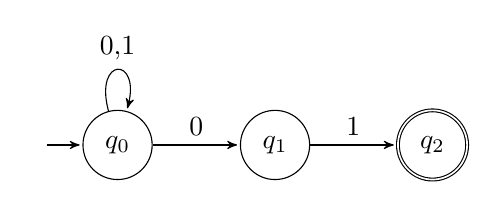
\begin{tikzpicture}[>=stealth',shorten >=1pt,auto,node distance=2cm]
                \node[initial,state] (q0)      {$q_0$};
                \node[state] (q1)  [right of=q0]     {$q_1$};
                \node[state,accepting] (q2) [right of=q1]     {$q_2$};
                \path[->]
                    (q0)  edge[loop above]  node {0,1} (q0)
                    (q0)  edge  node {0} (q1)
                    (q1)  edge node {1} (q2);
            \end{tikzpicture}
        }

        \column{0.4\textwidth}

        \begin{tabular}{r||c|c}
            $\delta$ & 0 & 1\\ \hline \hline		
            $\rightarrow q_0$ & $\{q_0,q_1\}$ & $\{q_0\}$\\ \hline 
            $q_1$ & $\emptyset$ & $\{q_2\}$\\ \hline 
            $*q_2$ & $\emptyset$ & $\emptyset$
        \end{tabular}        
        
    \end{columns}
        
    \bigskip\bigskip

    Processing the input $w=00101$:
    
    \begin{center}
        \scalebox{0.95}{
            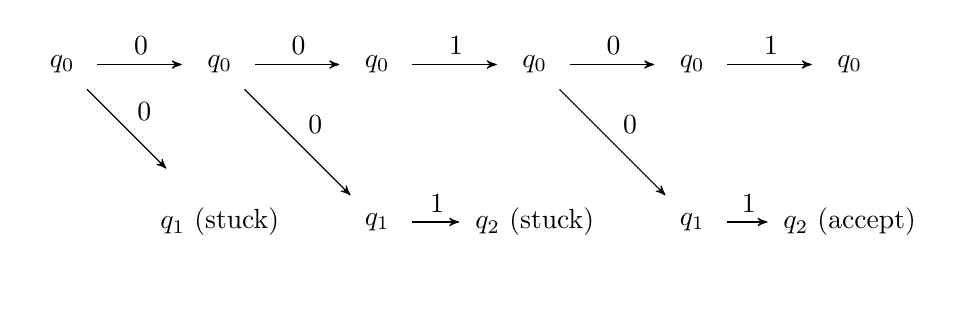
\begin{tikzpicture}[>=stealth',shorten >=1pt,auto,node distance=2cm]
                \tikzstyle{every state}=[draw=none]
                \node[state] (q0)      {$q_0$};
                \node[state] (q01)  [right of=q0]     {$q_0$};
                \node[state] (q02)  [right of=q01]     {$q_0$};
                \node[state] (q03)  [right of=q02]     {$q_0$};
                \node[state] (q04)  [right of=q03]     {$q_0$};
                \node[state] (q05)  [right of=q04]     {$q_0$};
                \node[state] (q11)  [below of=q01]     {$q_1$ (stuck)};
                \node[state] (q12)  [below of=q02]     {$q_1$};
                \node[state] (q13)  [below of=q04]     {$q_1$};
                \node[state] (q21)  [below of=q03]     {$q_2$ (stuck)};
                \node[state] (q22)  [below of=q05]     {$q_2$ (accept)};
                \path[->]
                    (q0)  edge  node {0} (q01)
                    (q01)  edge  node  {0} (q02)
                    (q02)  edge  node  {1} (q03)
                    (q03)  edge  node {0}  (q04)
                    (q04)  edge  node {1}  (q05)
                    (q0)  edge  node {0}  (q11)
                    (q01)  edge  node {0} (q12)
                    (q03)  edge  node {0} (q13)
                    (q12)  edge  node {1} (q21)
                    (q13)  edge  node {1} (q22);
            \end{tikzpicture}            
        }
    \end{center}

\end{frame}


\begin{frame}{The definition}

    \begin{definition}[Nondeterministic finite automation]
        An \alert{NFA} is a structure $A=(Q,\Sigma,\delta,S_0,F)$ consisting of:
        \begin{itemize}
            \item A finite set of \alert{states}, often denoted $Q$.
            \item A finite set of \alert{input symbols}, denoted $\Sigma$.
            \item A \alert{transition function} $\delta: Q \times \Sigma \rightarrow {\mathcal P}(Q)$ which returns \alert{a subset of $Q$}.
            \item A \alert{set of starting states} $S_0\subseteq Q$ (alternatively, only $q_0\in Q$).
            \item A   \alert{set accepting states} (final states) $F\subseteq Q$.
        \end{itemize}
    \end{definition}
    
\end{frame}


\begin{frame}{Extended transition function}

    \begin{definition}[$\delta^*$ for NFA]
    $\delta^*:Q\times \Sigma^*\rightarrow {\mathcal P}(Q)$, i.e. takes a state $q$ and a word $w$ and returns a set of states, and is defined by induction:
    \begin{itemize}
        \item $\delta^*(q,\epsilon)=\{q\}$.
        \item $\delta^*(q,ua)=\bigcup_{p\in\delta^*(q,u)}\delta(p,a)$ for $u\in\Sigma^*,a\in\Sigma$
    \end{itemize}
    (That is, it outputs the set of states to which there exists some path from $q$ with edges labelled $w$.)
    \end{definition}

    \bigskip
    
    \begin{columns}

        \column{0.6\textwidth}

        \small

        \begin{tabular}{ l @{=} c @{=}l}
            $\delta^*(q_0,\epsilon)$ &  & $\{q_0\} $\\ \hline
            $\delta^*(q_0,0)$ & $\delta(q_0,0)$ & $\{q_0,q_1\} $\\ \hline
            $\delta^*(q_0,00)$& $\delta(q_0,0)\cup \delta(q_1,0)$ & $\{q_0,q_1\} $\\ \hline
            $\delta^*(q_0,001)$ & $\delta(q_0,1)\cup \delta(q_1,1)$ & $\{q_0,q_2\} $\\ \hline
            $\delta^*(q_0,0010)$ & $\delta(q_0,0)\cup \delta(q_2,0)$ & $\{q_0,q_1\} $\\ 	\hline
            $\delta^*(q_0,00101)$ & $\delta(q_0,1)\cup \delta(q_1,1)$ & $\{q_0,q_2\} $
        \end{tabular}

        \column{0.4\textwidth}

        \scalebox{0.65}{
            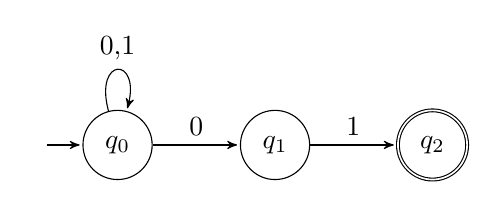
\begin{tikzpicture}[>=stealth',shorten >=1pt,auto,node distance=2cm]
                \node[initial,state] (q0)      {$q_0$};
                \node[state] (q1)  [right of=q0]     {$q_1$};
                \node[state,accepting] (q2) [right of=q1]     {$q_2$};
                \path[->]
                    (q0)  edge[loop above]  node {0,1} (q0)
                    (q0)  edge  node {0} (q1)
                    (q1)  edge node {1} (q2);
            \end{tikzpicture}
        }

    \end{columns}

\end{frame}


\begin{frame}{The language recognized}

    \begin{definition}[Language of an NFA]
        The language \alert{recognized by} an NFA $A=(Q,\Sigma,\delta,S_0,F)$: 
        $$
        \alert{L(A)}=\{w\in \Sigma^* \mid \delta^*(q_0,w)\cap F\neq \emptyset\text{ for some }q_0\in S_0\}
        $$        
    \end{definition}

    That is, we can get from some starting to some accepting state. 

    \bigskip

    \begin{example}
        The NFA from above indeed recognizes $L=\{w \mid w \hbox{ ends in 01}\} $. Prove by induction that $\delta^*(q_0,w)$:
        \begin{itemize}
            \item contains $q_0$ for every $w$
            \item contains $q_1$ iff $w$ ends in $0$
            \item contains $q_2$ iff $w$ ends in $01$
        \end{itemize}
    \end{example}


\end{frame}


\begin{frame}{Remarks}

    \begin{itemize}
        \item Abusing notation, for $S\subseteq Q$ we could (but won't) write $\delta^*(S,w)$ meaning $\bigcup_{q\in S}\delta^*(q,w)$. Then we would have:
        \begin{align*}
            &\delta^*(S,ua)=\delta(\delta^*(S,u),a) \\
            &L(A)=\{w\in\Sigma^*\mid\delta^*(S_0,w)\cap F\neq\emptyset\}
        \end{align*}
        
        \item The indistinguishable states/reduction algorithm fails for NFA:
        
        \begin{minipage}{0.35\linewidth}
            \scalebox{0.65}{
                    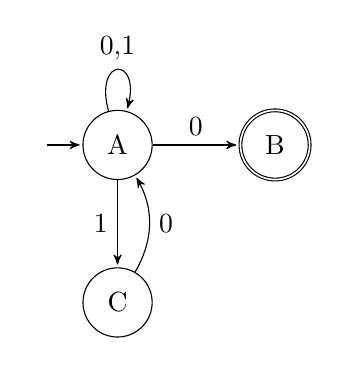
\begin{tikzpicture}
                        \node[initial,state] (a)    {A};
                        \node[state,accepting] (b)  [right of=a]     {B};
                        \node[state] (c) [below of=a]    {C};
                        \path[->]
                            (a)  edge[loop above]  node {0,1} (a)
                            (a)  edge  node {0} (b)
                            (a)  edge  node[swap] {1} (c)
                            (c)  edge[bend right]  node[swap] {0} (a)
                        ;
                    \end{tikzpicture}
            }            
        \end{minipage}
        \begin{minipage}{0.55\linewidth}
            we can remove $C$ but $\{A,C\}$ are distinguishable by $w=0$
        \end{minipage}
        
        \medskip
        \item Minimizing NFA is not easy, we could use exhaustive search        
    \end{itemize}

\end{frame}


\begin{frame}{Computation graph of a [D/N]FA}

    \begin{itemize}
        \item a \alert{configuration} is a pair $(q,v)$ where $q\in Q$ is the current state and $v\in\Sigma^*$ is the remaining (unread) input
        \item the \alert{computation graph} has all configurations as nodes and its oriented edges denote possible 1-step transitions, i.e. for NFA: $$(p,au)\to(q, u)\ \text{ iff }\ q\in \delta(p,a)$$
        \item accept iff path from some initial to some accepting config
        \item useful theoretical concept, not to be explicitly constructed
        \item later for other types of automata (configs more complex)
        \item similarly the \alert{computation tree} for input $w$: root is $(q_0,w)$, nodes labelled by configs (but do not identify same labels)        
    \end{itemize}

\end{frame}


\section*{Equivalence of NFA and DFA}


\begin{frame}{}

    Every DFA $D=(Q,\Sigma,\delta,q_0,F)$ can be trivially transformed to an equivalent NFA $N=(Q,\Sigma,\delta',\{q_0\},F)$, where \alert{$\delta'(q,a)=\{\delta(q,a)\}$}

    \bigskip

    Every NFA can also be transformed to an equivalent DFA albeit with a different, potentially \alert{exponentially bigger} set of states: using the \alert{subset construction}

    \bigskip

    Why NFA? Easier to design, usually no need to explicitly transform.

\end{frame}


\begin{frame}{Subset construction}

    Given $N=(Q_N,\Sigma,\delta_N,S_0,F_N)$ construct $D=(Q_D,\Sigma,\delta_D,q_0,F_D)$

    \begin{itemize}
        \item \alert{$Q_D={\mathcal P}(Q_N)$} (all subsets of $Q_N$) or discard those that would be unreachable: start constructing from the initial state
        \item \alert{$\delta_D(S,a)=\bigcup_{p \in S}\delta_N(p,a)$} for $S\subseteq Q_N$, $a\in \Sigma$ 
        \item \alert{$q_0=S_0$} (which is an element of $Q_D$)
        \item \alert{$F_D=\{S\subseteq Q_N \mid S \cap F_N \neq \emptyset\}$} (accept if contains accepting)
    \end{itemize}

    \begin{theorem}
        The resulting DFA $D$ is indeed equivalent to the original NFA $N$.
    \end{theorem}

    \begin{proof}
        By induction, show that $\delta^*_D(q_0,w)=\bigcup_{q\in S_0}\delta^*_N(q,w)$.
    \end{proof}

\end{frame}
    

\begin{frame}{Example of the subset construction}

    \scalebox{1}{
        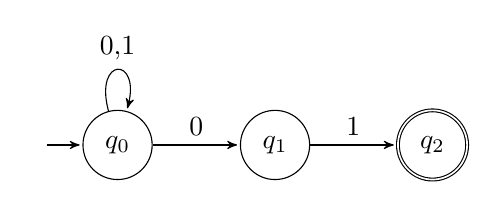
\begin{tikzpicture}[>=stealth',shorten >=1pt,auto,node distance=2cm]
            \node[initial,state] (q0)      {$q_0$};
            \node[state] (q1)  [right of=q0]     {$q_1$};
            \node[state,accepting] (q2) [right of=q1]     {$q_2$};
            \path[->]
                (q0)  edge[loop above]  node {0,1} (q0)
                (q0)  edge  node {0} (q1)
                (q1)  edge node {1} (q2);
        \end{tikzpicture}    
    }

    \vspace{24pt}

    \begin{columns}

        \column{0.6\textwidth}

        \scalebox{0.9}{
            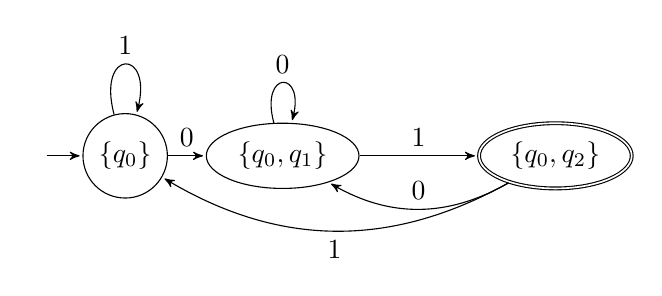
\begin{tikzpicture}[>=stealth',shorten >=1pt,auto,node distance=2cm]
                \node[initial,state] (q0)      {$\{q_0\}$};
                \node[elliptic state] (q1)  [right of=q0]     {$\{q_0,q_1\}$};
                \node[elliptic state,accepting] (q2) [right=1.5cm of q1]     {$\{q_0,q_2\}$};
                \path[->]
                    (q0)  edge[loop above]  node {1} (q0)
                    (q0)  edge  node {0} (q1)
                    (q1)  edge[loop above]  node {0} (q0)
                    (q1)  edge node {1} (q2)
                    (q2)  edge[bend left] node[swap] {0} (q1)
                    (q2)  edge[bend left] node {1} (q0)
                ;
            \end{tikzpicture}
        }
        
        \column{0.4\textwidth}

        \scriptsize

        \begin{tabular}{r || c | c}
            & 0  & 1\\ \hline \hline
            $\emptyset$ & $\emptyset$ &$\emptyset$ \\ 
            $\rightarrow \{q_0\}$ & $ \{q_0,q_1\}$ & $\{q_0\}$\\
            $\{q_1\}$ & $ \emptyset$ & $\{q_2\}$\\
            $*\{q_2\}$ & $ \emptyset$ & $ \emptyset$\\
            $\{q_0,q_1\}$ & $ \{q_0,q_1\}$ & $\{q_0,q_2\}$\\
            $*\{q_0,q_2\}$ & $ \{q_0,q_1\}$ & $\{q_0\}$\\
            $*\{q_1,q_2\}$ & $ \emptyset$ & $\{q_2\}$\\
            $*\{q_0,q_1,q_2\}$ & $ \{q_0,q_1\}$ & $\{q_0,q_2\}$
        \end{tabular}
        
    \end{columns}

\end{frame}


\begin{frame}{Sometimes it blows up}
    
    \begin{example}[Hard case for the subset construction]
        Words over $\{0,1\}$ where the $n$th symbol from the end is 1.
    \end{example}
    
    Intuitively, a DFA must remember the last $n$ symbols it has read.
    
    \begin{center}
        \scalebox{0.9}{
            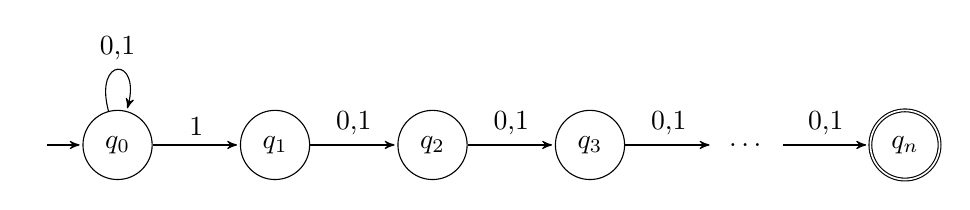
\begin{tikzpicture}[>=stealth',shorten >=1pt,auto,node distance=2cm]
                \node[initial,state] (q0)      {$q_0$};
                \node[state] (q1)  [right of=q0]     {$q_1$};
                \node[state] (q2)  [right of=q1]     {$q_2$};
                \node[state] (q3)  [right of=q2]     {$q_3$};
                \node[state] (q5)  [draw=none,right of=q3]     {\ldots};
                \node[state,accepting] (q6) [right of=q5]     {$q_n$};
                \path[->]
                    (q0)  edge[loop above]  node {0,1} (q0)
                    (q0)  edge  node {1} (q1)
                    (q1)  edge node {0,1} (q2)
                    (q2)  edge node {0,1} (q3)
                    (q3)  edge node {0,1} (q5)
                    (q5)  edge node {0,1} (q6)
                ;
            \end{tikzpicture}                
        }
    \end{center}

    \bigskip

    \begin{exercise}
        Prove that any DFA recognizing the langauge has $\Omega(2^n)$ states.
    \end{exercise}
    (Hint: Use the Myhill--Nerode theorem.)

\end{frame}


\section*{Adding $\epsilon$-transitions}


\begin{frame}{$\epsilon$-transitions are useful and not too much hassle}

    It is sometimes useful to further generalize NFAs by allowing \alert{$\epsilon$-transitions}, i.e., change state without reading any input symbol.

    \bigskip

    In an \alert{$\epsilon$-NFA}, the transition function is $\delta:Q \times (\Sigma\cup \{\epsilon\})\to\mathcal{P}(Q)$
    
    \bigskip

    The subset construction still works, if we restrict to subsets closed under $\epsilon$-transitions.

    \bigskip

    \begin{definition}[$\epsilon$-NFA]
        A \alert{$\epsilon$-NFA} is $E=(Q,\Sigma,\delta,S_0,F)$, where all components have the same interpretation as for NFAs, except that $\delta$ is now a function that takes arguments from $Q \times (\Sigma\cup \{\epsilon\})$. (We require $\epsilon \notin \Sigma$.)
    \end{definition}

\end{frame}


\begin{frame}{Example: decimal numbers}

    \begin{enumerate}[(1)]
        \item Optionally a + or - sign, then
        \item a string of digits, then
        \item a decimal point, and
        \item another string of digits. 
    \end{enumerate}
    At least one of strings (2) and (4) must be nonempty.

    \begin{columns}

        \column{0.6\textwidth}

        \begin{center}
            \scalebox{0.85}{
                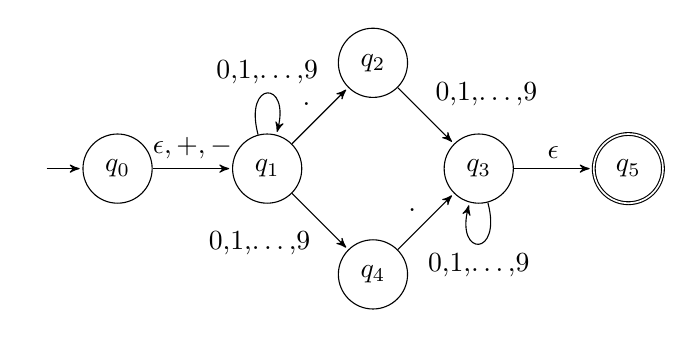
\begin{tikzpicture}[>=stealth',shorten >=1pt,auto,node distance=1.9cm]
                    \node[initial,state] (q0)      {$q_0$};
                    \node[state] (q1)  [right of=q0]     {$q_1$};
                    \node[state] (q2)  [above right of=q1]     {$q_2$};
                    \node[state] (q3)  [below right of=q2]     {$q_3$};
                    \node[state] (q4)  [below right of=q1]     {$q_4$};
                    \node[state,accepting] (q5)  [right of=q3]     {$q_5$};
                    \path[->]
                        (q0)  edge  node {$\epsilon,+,-$} (q1)
                        (q1)  edge[loop above]  node {0,1,\ldots,9} (q1)
                        (q3)  edge[loop below]  node {0,1,\ldots,9} (q3)
                        (q1)  edge node {.} (q2)
                        (q2)  edge node {0,1,\ldots,9} (q3)
                        (q4)  edge node {.} (q3)
                        (q3)  edge node {$\epsilon$} (q5)
                        (q1)  edge[swap] node {0,1,\ldots,9} (q4)
                        ;
                \end{tikzpicture}
            }
        \end{center}
    
        \column{0.4\textwidth}

        \tiny

        \begin{center}
            \begin{tabular}{c || l | l | l | l}
                & $\epsilon$ & `+',`-' & `.' & `0',`1',\ldots,`9'\\ \hline \hline
                $q_0$ & $\{q_1\}$ & $\{q_1\}$ & $\emptyset$& $\emptyset$\\
                $q_1$  & $\emptyset$& $\emptyset$& $\{q_2\}$ & $\{q_1,q_4\}$\\
                $q_2$  & $\emptyset$& $\emptyset$& $\emptyset$& $\{q_3\}$\\
                $q_3$  & $\{q_5\}$& $\emptyset$& $\emptyset$& $\{q_3\}$\\
                $q_4$  & $\emptyset$& $\emptyset$& $\{q_3\}$& $\emptyset$\\
                $q_5$ & $\emptyset$& $\emptyset$& $\emptyset$& $\emptyset$
            \end{tabular}  
        \end{center}      
        
    \end{columns}
        
\end{frame}


\begin{frame}{$\epsilon$-closure and $\delta^*$}

    For $S\subseteq Q$ define the \alert{$\epsilon$-closure} of $S$ recursively as follows:
    \begin{itemize}
        \item $S\subseteq\epsilon CLOSE(S)$
        \item if $p\in \epsilon CLOSE(S)$ and $r \in \delta(p,\epsilon)$ then $r \in \epsilon CLOSE(S)$
    \end{itemize}

    The extended transition function is then naturally defined:

    \begin{definition}[$\delta^*$ for $\epsilon$-NFA]
        For an $\epsilon$-NFA $E=(Q,\Sigma,\delta,S_0,F)$ define $\delta^*$ inductively:
        \begin{itemize}
            \item $\delta^*(q,\epsilon)=\epsilon CLOSE(\{q\})$
            \item $\delta^*(q,ua)=\epsilon CLOSE\left(\bigcup_{p\in\delta^*(q,u)} \delta(p,a)\right)$ for $u\in \Sigma^*, a\in \Sigma$        
        \end{itemize}
    \end{definition}

    $\delta^*(q,w)$ still means states we can be in if start from $q$ and read $w$


    
\end{frame}


\begin{frame}{Example continued}

    \vspace{0.5cm}

    \begin{flushright}
        \scalebox{0.7}{
            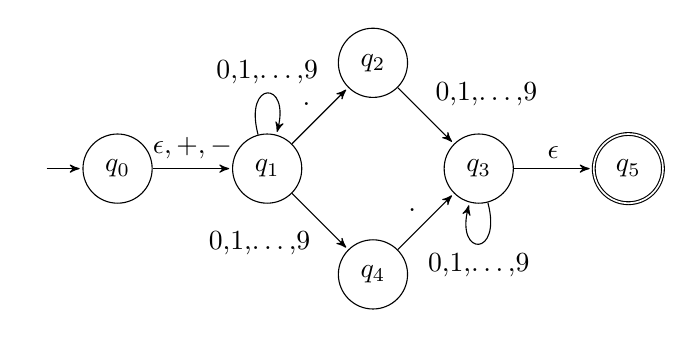
\begin{tikzpicture}[>=stealth',shorten >=1pt,auto,node distance=1.9cm]
                \node[initial,state] (q0)      {$q_0$};
                \node[state] (q1)  [right of=q0]     {$q_1$};
                \node[state] (q2)  [above right of=q1]     {$q_2$};
                \node[state] (q3)  [below right of=q2]     {$q_3$};
                \node[state] (q4)  [below right of=q1]     {$q_4$};
                \node[state,accepting] (q5)  [right of=q3]     {$q_5$};
                \path[->]
                    (q0)  edge  node {$\epsilon,+,-$} (q1)
                    (q1)  edge[loop above]  node {0,1,\ldots,9} (q1)
                    (q3)  edge[loop below]  node {0,1,\ldots,9} (q3)
                    (q1)  edge node {.} (q2)
                    (q2)  edge node {0,1,\ldots,9} (q3)
                    (q4)  edge node {.} (q3)
                    (q3)  edge node {$\epsilon$} (q5)
                    (q1)  edge[swap] node {0,1,\ldots,9} (q4)
                    ;
            \end{tikzpicture}
        }
    \end{flushright}

    \vspace{-4cm}
    
    $\epsilon$-closure:
    \begin{itemize}
        \item $\epsilon CLOSE(\{q_0\}) = \{q_0,q_1\}$
        \item $\epsilon CLOSE(\{q_1\}) = \{q_1\}$
        \item $\epsilon CLOSE(\{q_3\}) = \{q_3,q_5\}$
        \item $\epsilon CLOSE(\{q_3,q_4\}) = \{q_3,q_4,q_5\}$
    \end{itemize}

    Extended transition function: $\delta^*(q_0,5.6)$
    
    \begin{itemize}
        \item $\delta^*(q_0,\epsilon) = \epsilon CLOSE(\{q_0\}) = \{q_0,q_1\}$
        \item $\delta^*(q_0,5) = \epsilon CLOSE(\bigcup\nolimits_{q \in \delta^*(q,\epsilon)}\delta(q,5)) = \epsilon CLOSE(\delta(q_0,5)\cup \delta(q_1,5)) = \{q_1,q_4\}$
        \item $\delta^*(q_0,5.) = \epsilon CLOSE(\delta(q_1,.)\cup \delta(q_4,.)) = \{q_2,q_3,q_5\}$
        \item $\delta^*(q_0,5.6) = \epsilon CLOSE(\delta(q_2,6)\cup \delta(q_3,6)\cup \delta(q_5,6)) = \{q_3,q_5\}$
    \end{itemize}

\end{frame}


\begin{frame}{Equivalence of $\epsilon$-NFA and DFA}

    Add $\epsilon$-closure to the subset construction: 
    
    Given an $\epsilon$-NFA $E=(Q_E,\Sigma,\delta_E,S_0,F_E)$ construct a DFA $D=(Q_D,\Sigma,\delta_D,q_0,F_D)$

    \begin{itemize}
        \item $Q_D=\{S\subseteq Q_E\mid \alert{S=\epsilon CLOSE(S)}\}$, i.e., only \alert{$\epsilon$-closed} subsets
        \item $\delta_D(S,a)=\alert{\epsilon CLOSE(}\bigcup_{p \in S}\delta_E(p,a)\alert{)}$
        \item $q_0=\alert{\epsilon CLOSE(}S_0\alert{)}$
        \item $F_D=\{S\in Q_D \mid S \cap F_E \neq \emptyset\}$, i.e., $\epsilon$-closed subsets containing some accepting state
    \end{itemize}

    \begin{theorem}
        A language $L$ is recognized by an $\epsilon$-NFA, iff $L$ is regular.
    \end{theorem}    
    (Proof similar as for NFA.)

\end{frame}


\section{1.7 Closure properties}


\section{Set operations}


\begin{frame}{Set operations preserving regularity}

    For languages $L, M$:
    \begin{itemize}
        \item \alert{complement} $\overline{L}= -L=\{w\mid w\notin L\}=\Sigma^*\setminus L$
        \item \alert{intersection} $L\cap M=\{w\mid w\in L\ \text{ and }\ w\in M\}$
        \item \alert{union} $L\cup M=\{w\mid w\in L\ \text{ or }\  w\in M\}$
        \item \alert{difference} $L- M=\{w\mid w\in L \ \text{ and }\  w\notin M\}$
    \end{itemize}

    \begin{theorem}[Closure under set operations]
        Given a pair of regular languages $L$ and $M$, the languages $\overline{L}$, $L\cap M$, $L\cup M$, and $L- M$ are also regular.
    \end{theorem}

    Note: union/intersection of \alert{infinitely many} regular languages is generally not regular!

    % \begin{example}\small
    %     \begin{itemize}
    %         \item complement: words that do not end with `a'
    %         \item intersection: words of even length that end with  `baa'
    %         \item union: words that start with `aab' or end with `baa'            
    %         \item difference: words of even length that do not end with `baa'            
    %     \end{itemize}
    % \end{example}

\end{frame}


\begin{frame}{Proof}

    We can assume that $L,M$ are over the same alphabet $\Sigma$. Let $L=L(A),M=L(B)$ for DFA $A,B$. Ensure that their transition functions are total (if not, add a fail state).
    \begin{itemize}
        \item \alert{complement}: accepted by the DFA $A'$ obtained from $A$ by switching accepting and nonaccepting states: $F_{A'}=Q_A\setminus F_A$
        \item \alert{intersection}: accepted by the \alert{product automaton}
        \begin{align*}
            & C=A\times B=(Q_A\times Q_B,\Sigma,\delta_C,({q_0}_A,{q_0}_B),F_A\times F_B)\\
            & \delta_C((q_A,q_B),a)=(\delta_A(q_A,a),\delta_B(q_B,a))            
        \end{align*}    
        \item \alert{union}: by De Morgan laws, $L \cup M=\overline{\overline{L}\cap \overline{M}}$
        \item \alert{difference}: $L-M=L\cap \overline{M}$\hfill\qedsymbol
    \end{itemize}
    
    Note: For union and difference we can also directly construct the product automaton but with $F_C=(F_A\times Q_B)\cup(Q_A\times F_B)$ and $F_C=F_A\times Q_B$, respectively.

\end{frame}


\begin{frame}{Example of the constructions}

    Complement: words not ending in $01$
    \begin{center}
        \scalebox{0.8}{
            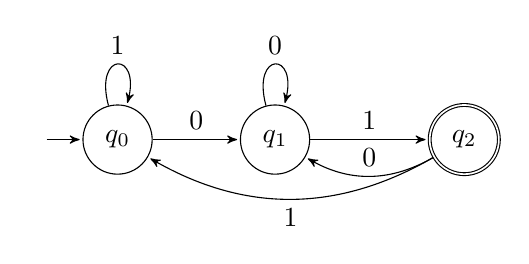
\begin{tikzpicture}[>=stealth',shorten >=1pt,auto,node distance=2cm]
                \node[initial,state] (q0)      {$q_0$};
                \node[state] (q1)  [right of=q0]     {$q_1$};
                \node[state, accepting] (q2) [right=1.5cm of q1]     {$q_2$};
                \path[->]
                    (q0)  edge[loop above]  node {1} (q0)
                    (q0)  edge  node {0} (q1)
                    (q1)  edge[loop above]  node {0} (q0)
                    (q1)  edge node {1} (q2)
                    (q2)  edge[bend left] node[swap] {0} (q1)
                    (q2)  edge[bend left] node {1} (q0)
                    ;
            \end{tikzpicture}  
            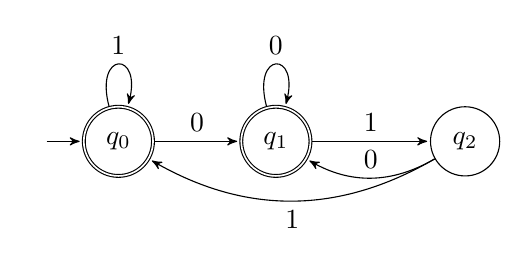
\begin{tikzpicture}[>=stealth',shorten >=1pt,auto,node distance=2cm]
                \node[initial,state, accepting] (q0)      {$q_0$};
                \node[state, accepting] (q1)  [right of=q0]     {$q_1$};
                \node[state] (q2) [right=1.5cm of q1]     {$q_2$};
                \path[->]
                    (q0)  edge[loop above]  node {1} (q0)
                    (q0)  edge  node {0} (q1)
                    (q1)  edge[loop above]  node {0} (q0)
                    (q1)  edge node {1} (q2)
                    (q2)  edge[bend left] node[swap] {0} (q1)
                    (q2)  edge[bend left] node {1} (q0)
                    ;
            \end{tikzpicture}    
        }
    \end{center}
    
    \vspace{-6pt}
    Intersection: words containing both 0 and 1
    \vspace{-6pt}

    \begin{center}
        \scalebox{0.8}{
            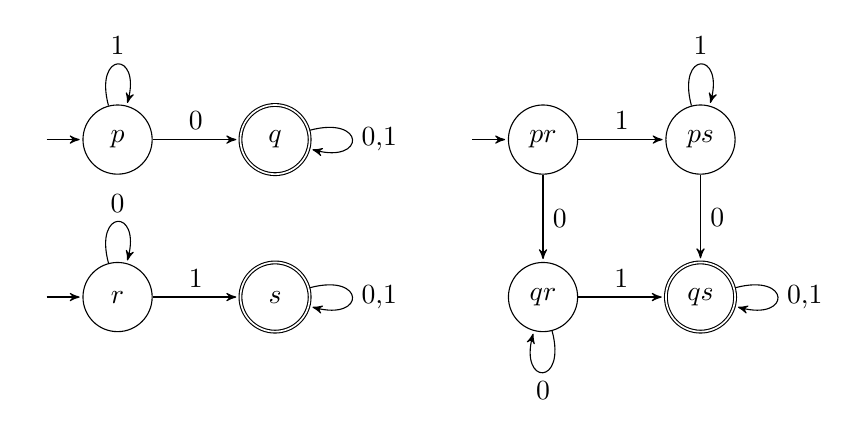
\begin{tikzpicture}                
                \node[initial,state] (p)      {$p$};
                \node[state, accepting] (q)  [right of=p]     {$q$};
                \node[initial,state] (r)  [below of=p]    {$r$};
                \node[state, accepting] (s)  [right of=r]     {$s$};
                \node[initial,state] (pr)   [right=2.5cm of q]   {$pr$};
                \node[state] (ps)  [right of=pr]     {$ps$};
                \node[state] (qr)  [below of=pr]    {$qr$};
                \node[state, accepting] (qs)  [right of=qr]     {$qs$};
                \path[->]
                    (p)  edge[loop above]  node {1} (p)
                    (p)  edge  node {0} (q)
                    (r)  edge[loop above]  node {0} (r)
                    (r)  edge  node {1} (s)
                    (s)  edge[loop right]  node {0,1} (s)
                    (q)  edge[loop right]  node {0,1} (q)
                    (ps)  edge[loop above]  node {1} (ps)
                    (pr)  edge  node {0} (qr)
                    (ps)  edge  node {0} (qs)
                    (qr)  edge[loop below]  node {0} (qr)
                    (qr)  edge  node {1} (qs)
                    (pr)  edge  node {1} (ps)
                    (qs)  edge[loop right]  node {0,1} (qs)
                    ;
            \end{tikzpicture}    
        }
    \end{center}    

\end{frame}


\begin{frame}{Applications}

    \begin{example}
        Accepting words with $3k+2$ of $1$'s and no substring $11$.
    \end{example}
    \begin{itemize}
        \item The direct construction is complicated.
        \item $L_1=\{w\in\{0,1\}^* \mid |w|_1=3k+2\}$
        \item $L_2=\{w\in\{0,1\}^* \mid w=u11v\text{ for some }u,v\in\{0,1\}^*\}$
        \item $L=L_1-L_2$.
    \end{itemize}   
    
    \bigskip
        
    \begin{example}
        The language $M=\{w\in\{0,1\}^* \mid |w|_0\neq |w|_1\}$ is not regular.
    \end{example}
    \begin{itemize}
        \item If  $M$ is regular, then $\overline{M}$ is also regular.
        \item We know $\overline{M}$ is not regular (Pumping lemma).
        \item So $M$ cannot be regular.
    \end{itemize}

\end{frame}  


\begin{frame}{One more application}

    \begin{example}
        The language $L_{0\neq 1}=\{0^i1^j\mid i\neq j, i,j\in\mathbb N\}$ is not regular:
    \end{example}
    \begin{itemize}
        \item The language $L_{01}=\{0^i1^j\mid i,j\in\mathbb N\}$ is regular (we can construct a DFA directly).
        \item A difference of two regular languages is regular.
        \item $L_{01}$ is regular. Assume that $L_{0\neq 1}$ is regular, then $L_{01}-L_{0\neq 1}=\{0^i1^i\mid i\in\mathbb N\}$ is also regular.
        \item But it is not regular (Pumping lemma)---a contradiction.
    \end{itemize}

\end{frame}


\section{String operations}


\begin{frame}{String operations preserving regularity}
    
    \begin{itemize}
        \item \alert{concatenation} $L.M=\{uv\mid u\in L\text{ and }v\in M\}$, we also write $L.w=L.\{w\}$ and $w.L=\{w\}.L$ for $w\in \Sigma^*$
        \item \alert{powers} of languages $L^0=\{\epsilon\}$, $L^{i+1}=L^i.L$
        \item \alert{iteration} $L^*=L^0\cup L^1\cup L^2 \ldots=\bigcup_{i\geq 0}L^i$
        \item \alert{positive iteration} $L^+=L^1\cup L^2 \ldots=\bigcup_{i\geq 1}L^i$
        
        that is, $L^*=L^+\cup \{\epsilon\}$
        \item \alert{reverse} $L^R=\{u^R| u\in L\}$, $(x_1x_2\ldots x_n)^R=x_nx_{n-1}\ldots x_2x_1$
        \item \alert{left quotient} of $L$ with $M$,  $M\setminus L=\{v|uv\in L\text{ and }u\in M\}$
        \item \alert{left derivation} of $L$ with $w$, $\partial_w L=\{w\}\setminus L$
        \item \alert{(right) quotient} of $L$ with $M$, $L/ M=\{u|uv\in L\text{ and }v\in M\}$
        \item \alert{right derivation} of $L$ with $w$$\partial_w^R L=L/\{w\}$
    \end{itemize}
\end{frame}


\begin{frame}{Regular languages are closed under those}

    \begin{theorem}[Closure under string operations]
        Given a pair of regular languages $L$ and $M$, the languages $L.M$, $L^*$, $L^+$, $L^R$, $M\backslash L$, and $L/M$ are also regular.
    \end{theorem}

    We assume that we have DFA for $L$ and $M$ with disjoint sets of states and that any newly added states are indeed new (otherwise rename states)

    We give constructions of $\epsilon$-NFA or NFA for each operation.

\end{frame}


\begin{frame}{Proof for concatenation $L.M$}

    Let $A_1=(Q_1,\Sigma, \delta_1,q_1,F_1)$ and $A_2=(Q_2,\Sigma, \delta_2,q_2,F_2)$ be DFA such that $L=L(A_1)$ and $M=L(A_2)$. Assume that $\delta_1,\delta_2$ are total functions and $Q_1\cap Q_2=\emptyset$.
    
    Define an $\epsilon$-NFA $B=(Q_1\cup Q_2,\Sigma,\delta,\{q_1\},F_2)$, where:
    \begin{itemize}
        \item $\delta(q,a)=\{\delta_1(q,a)\}$ for $q\in Q_1,a\in\Sigma$,
        \item $\delta(q,a)=\{\delta_2(q,a)\}$ for $q\in Q_2,a\in\Sigma$,
        \item $\delta(q,\epsilon)=\{q_2\}$ for $q\in F_1$
    \end{itemize}
    (And $\delta(q,x)=\emptyset$ in all other cases.)
    
    It is straightforward to verify that $L(B)=L(A_1).L(A_2)$.\hfill\qedsymbol

    % Let $A_1=(Q_1,\Sigma, \delta_1,q_1,F_1)$ and $A_2=(Q_2,\Sigma, \delta_2,q_2,F_2)$ be DFA such that $L=L(A_1)$ and $M=L(A_2)$.
    
    % Define an $\epsilon$-NFA $B=(Q\mathbin{\dot\cup} \{q_0\},\Sigma,\delta,\{q_0\},F_2)$ (note that we end after reading the word in the second language $M$) where:
    % \begin{align*}
    % &\delta(q_0,x)=\emptyset\text{ for }x\in \Sigma\\
    % &\delta(q_0,\epsilon)=\begin{cases}
    % \{q_1,q_2\}&\text{for }q_1\in F_1\hfill\text{ (i.e. if $\epsilon\in L(A_1)$)}\\
    % \{q_1\}&\text{for }q_1\notin F_1\hfill\text{ (i.e., if $\epsilon \notin L(A_1)$)}
    % \end{cases}\\
    % &\delta(q,x)=
    % \begin{cases}
    % \{\delta_1(q,x)\}&\text{for $q\in Q_1$ and $\delta_1(q,x)\notin F_1$ (stay in $A_1$)}\\
    % \{\delta_1(q,x),q_2\}&\text{for $q\in Q_1$ and $\delta_1(q,x)\in F_1$} \\ & \text{(nondeterministic transition from $A_1$ to $A_2$)}\\
    % \{\delta_2(q,x)\}&\text{for $q\in Q_2$  (stay in $A_2$)}
    % \end{cases}
    % \end{align*}
    % It is straightforward to verify that $L(B)=L(A_1).L(A_2)$.\hfill\qedsymbol

\end{frame}


\begin{frame}{Proof for iteration $L^*$, $L^+$}

    Let $A=(Q,\Sigma, \delta,q_0,F)$ be DFA such that $L=L(A)$. 
    \begin{itemize}
        \item \textbf{Idea:} repeated computation of $A=(Q,\Sigma, \delta,q_0,F)$, a nondeterministic decision whether to restart or continue.
        \item New (re-)start state $q_R$, accepting for $L^*$ but not for $L^+$.
    \end{itemize}
       
    Define an NFA $B=(Q\mathbin{\dot\cup}\{q_R\},\Sigma,\delta_B,\{q_R\},F_B$ where:
    \begin{itemize}
        \item $F_B=F\cup\{q_R\}$ for $L^*$, $F_B=F$ for $L^+$
        \item $\delta_B(q_R,\epsilon)=\{q_0\}$ \hfill start computation on $A$
        \item $\delta_B(f,\epsilon)=\{q_R\}$ for $f\in F$ \hfill nondeterministic restart
        \item $\delta_B(q,a)=\{\delta(q,a)\}$ for $q\in Q,a\in \Sigma$ \hfill computation of $A$
    \end{itemize}

    Then $L(B)=L(A)^*$ (if $q_R\in F_B$), or $L(B)=L(A)^+$ (if $q_R\notin F_B$).
    
    \hfill\qedsymbol

\end{frame}
    

\begin{frame}{Proof for reverse $L^R$}

    \textbf{Idea:} reverse edges in the state diagram; we get an NFA

    Given a DFA  $A=(Q,\Sigma, \delta,q_0,F)$ such that $L=L(A)$, define an NFA $B=(Q,\Sigma,\delta_B,F,\{q_0\})$, where:
    $$
        \delta_B(q,x)=\{p\mid \delta(p,x)=q\}
    $$

    Then for any word $w=x_1x_2\ldots x_n$:
    
    \begin{center}
        $q_0,q_1,q_2,\ldots, q_n$ is an accepting computation for $w$ in $A$   

        if and only if

        $q_n,q_{n-1},\ldots,q_2,q_1,q_0$ is an accepting computation for $w^R$ in $B$
    \end{center}
    \hfill\qedsymbol

    Note: $L$ is regular \alert{if and only if} $L^R$ is regular.

\end{frame}


\begin{frame}{Proof for quotients $M\setminus L$ and $L/ M$}

    

    \textbf{Idea for $M\setminus L$:} use an automaton for $A$ but start in states reachable from the initial state by a word in $M$. 
    
    Given a DFA  $A=(Q,\Sigma, \delta,q_0,F)$ such that $L=L(A)$, define an NFA $B=(Q,\Sigma,\delta',S,F)$ where $\delta'(q,a)=\{\delta(q,a)\}$ where $\delta'(q,a)=\{\delta(q,a)\}$ and
    $$
    S=\{q\in Q\mid q=\delta(q_0,u)\text{ for some }u\in M\}
    $$
    Note: $S$ can be found algorithmically: use $A_q=(Q,\Sigma, \delta,q_0,\{q\}))$, check if $L(A_q)\cap M\neq \emptyset$.
       
    $v\in M\setminus L$ $\Leftrightarrow$ $(\exists u\in M) uv\in L$ \\$\Leftrightarrow$ $(\exists u\in M)(\exists q \in Q)(\delta(q_0,u)\ \&\ \delta(q,v)\in F)$ \\$\Leftrightarrow$ $(\exists q \in S) \delta(q,v)\in F$ \\$\Leftrightarrow$ $v\in L(B)$

    To prove the claim for $L/ M$, note that $L/ M=(M^R\setminus L^R)^R$. \hfill\qedsymbol

\end{frame}


\begin{frame}{Summary of Lecture 3}

    \begin{itemize}
        \item Nondeterministic finite automata (NFA): can `guess' the right path to accepting, computation described by a state tree.
        \item $\epsilon$-transitions: allow to change states without reading any input
        \item Subset construction: every NFA and $\epsilon$-NFA is equivalent to a DFA (but can be easier to design, much smaller).
        \item Regular languages are closed under set operations (union, intersection, complement, difference)
        \item And under string operations (concatenation, iteration and positive iteration, reverse, left and right quotient)
    \end{itemize}

\end{frame}


\end{document}



